\chapter{Umsetzung}
\label{cha:Umsetzung}
Dieses Kapitel stellt den praktischen Teil der Projektarbeit dar. Es werden zunächst die Technologien, welche zur Umsetzung verwendet werden, dargestellt. Dann werden Hindernisse, auf die der Autor bei der Umsetzung stieß, dargelegt. Und schließlich wird auf das Konzept und dessen Implementierung eingegangen.

\section{Verwendete Technologien}
\label{sec:Umsetzung_usedtech}
Die Neuentwicklung der \ac{EEI} soll in SAP UI5 erstellt werden. SAP UI5 ist eine Sammlung von Entwicklungswerkzeugen der SAP SE für HTML5. Es unterstützt die Programmierung von Desktop- als auch mobilen Applikationen. Neben der Programmierung in HTML5 kann auch Quelltext in Javascript geschrieben, welcher clientseitig ausgeführt wird. \cite[S. 5]{SAPSE.2015} Durch die Nutzung von Webtechnologien, wie HTML und Javascript, sind die Applikationen, welche mit SAP UI5 gebaut werden, als webbasierte Technologien zu bezeichnen.

SAPUI5 wird bei dieser Entwicklung aus folgenden allgemeinen Gründen verwendet. Zum einen ist SAP UI5 der aktuelle Stand was Oberflächentechnologien bei der SAP SE angeht. Dadurch, dass es sich bei SAP UI5 um eine Technologie für webbasierte Applikationen handelt, ist eine Anwendung diesen Typs unabhängig vom Betriebsystem des Clients nutzbar. 

Außerdem spricht die clientseitige Ausführung von Javascript-Quelltext für die Nutzung von SAP UI5 bei der Neuentwicklung der \ac{EEI}. So kann zur Authentifizierung gegenüber dem Exchange Server die \ac{SSO}-Technologie \ac{IWA} verwendet werden. Serverseitiger Quelltext versuchte die Nutzerdaten per \ac{IWA} vom Nutzer des Servers zu beziehen. Dies machte keinen Sinn in diesem Kontext.
Wegen der Nutzung der \ac{IWA} bedarf es bei der Konsumierung der \ac{EEI} keiner separaten Authentifizierung oder einer Speicherung der Zugangsdaten zum Exchange Server.

Da der Quelltext der Datenübertragung in Javascript (siehe S. \pageref{cha:Beigaben}) geschrieben wird, wird für die Kommunikation mit \ac{EWS} auf das Konzept \ac{AJAX} (siehe Kapitel \ref{cha:WS_AJAX}) zurückgegriffen. (siehe Kapitel \ref{cha:Umsetzung_JS_XHR})

Die \ac{EWS} werden genutzt zur Datenübertragung zwischen \ac{EEI} und dem \ac{MS} Exchange Server, da dies die Übertragung allein durch die Nutzung von Standard Javascript Objekten ermöglicht. Es werden so keine zusätzlichen Javascript-Bibliotheken außerhalb der SAP UI5-Bibliotheken benötigt. Dies hat zum einen einen rechtlichen Vorteil beim späteren Verkauf dieser Lösung an Kunden, sorgt aber auch dafür, dass das Programm nicht unnötig kompliziert und aufgeblasen wird.

\section{Hindernisse bei der Umsetzung}
Die \ac{SOP} stellt ein wesentliches Hindernis beim Konsum der \ac{EWS} dar. Das Problem einer die Anwendung blockierenden \ac{SOP} ist zu beachten, da nicht davon auszugehen ist, dass innerhalb eines Unternehmen, welches \ac{EEI} einsetzt, das die Weboberfläche des \ac{CRM}-Systems und die \ac{EWS} über die exakt gleiche Domain zu erreichen sind.

Damit die \ac{SOP} nicht greift, muss der \ac{IIS}, in dessen Anwendungspool die \ac{EWS} verwaltet und bereitgestellt werden, dies über das Mitsenden eines bestimmten Header-Parameters verhindern. Für diese Konfiguration muss man Zugriff auf den \ac{MS} Windows Server haben, auf dem der jeweilige Exchange Server ausgeführt wird. Im Server-Manager des Windows Servers wählt man den passenden Server innerhalb der Konfiguration des \ac{IIS} (Rollen->WebServer (IIS)->Server auswählen) aus. Dort ist \ac{EWS} als eine Site des Servers aufgeführt. Diese wählt man aus und wählt dort die Option \emph{HTTP-Antwortheader}. Über \emph{Hinzufügen} fügt man die Zeile, welche die SOP unterdrückt hinzu. 

Name: 'Access-Control-Allow-Origin'; Wert: zu erlaubende Domain.

Zusätzlich ist für die Site zu den \ac{EWS} noch die Authentifizierungsmethode zu bestimmen. Unter dem Punkt Authentifizierung müssen alle Methoden außer der Methode \emph{Windows Authentifizierung} deaktiviert sein. Über Rechtsklick auf die aktivierte \emph{Windows Authentifizierung} muss unter \emph{Anbieter} der Wert \emph{Negotiate} an die oberste Stelle geschoben und damit Kerberos als Standardauthentifizierungsmethode festgelegt werden. \cite{Jaganathan.2006}

%\section{Konzept und Implementierung}
\pagebreak

\section{Konzept}
Das Konzept der Anwendung sieht eine Teilung des Abrufes der \ac{EWS} in drei Teile vor.
 
Zunächst wird die SOAP-Nachricht der Anfrage - im Quelltext Request Body genannt - generiert, welche im HTTP-Body des HTTP-Requests abgelegt wird. Abbildung \ref{fig:abb1} zeigt, welche zu welchen Funktionen es möglich sein soll einen Request Body zu erstellen. 

Mittels dieses Request Bodys wird über eine Methode (genannt ewsConnect, siehe Anhang \ref{subsec:meth_ewscon}), welche für alle Anfragen gleich ist, die Anfrage abgesetzt. Diese Methode gibt die Antwort zurück, die sie vom Webservice \ac{EWS} erhalten hat.

Da nicht alle Anfragen an \ac{EWS} auch eine Antwort über einen Fehlerbericht hinaus erwarten, gibt es eine Methode die zunächst diesen Fehlerbericht auswertet und für alle Anfragen gleich und somit generisch ist. Für die Anfragen, bei denen Informationen zurück erwartet werden, gibt es spezielle Methoden, welche die Informationen aus dem XML-Quelltext der SOAP-Antwortnachrichten extrahieren. Diese Informationen werden in \ac{JSON}-Objekte verpackt, dass sie einfach in Javascript zur Darstellung oder ähnlichen Zwecken weiterverarbeitet werden können. (siehe \ref{fig:abb1})

%Eine vollständige Anfrage an einen Webservice mittels dieser Methoden wird anhand des folgenden Codebeispiels verdeutlicht.


%\begin{lstlisting}[language=JavaScript]
%var vIdEmail = 'XYZ123';
%var vRequestBody = getRequestBodyGetEmail(vIdEmail);
%var vResponse = ewsConnect(vRequestBody);
%var vNoError  = processResponseGeneric(vResponse);
%if(vNoError){
% var vResult = processResponseGetEmail(vResponse);
%}

%\end{lstlisting} 
%(Für den Quelltext der hier aufgeführten Methoden siehe Anhang (S. \pageref{cha:attCodeEWSCONNECT}) bzw. Beigaben (S. \pageref{cha:Beigaben}))

\begin{figure}[htb]                     \centering 
	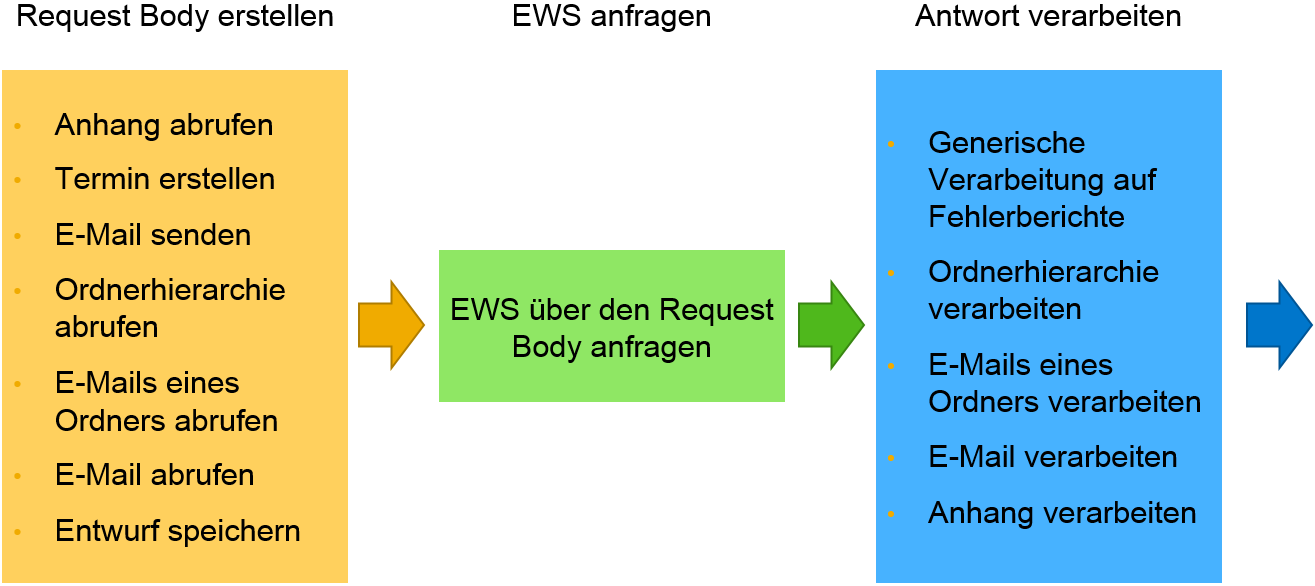
\includegraphics[width=1\linewidth]{Abbildungen/Konzept_ews_connect}
	\caption{Verdeutlichung des Konzepts} 
	\sc{Eigene Darstellung}
	\label{fig:abb1} 
\end{figure} 

\pagebreak

\section{Implementation}
\label{cha:Umsetzung_JS_XHR}
\ac{AJAX} ist als Basis der Kommunikation mit dem \ac{EWS} festgeschrieben. (siehe Kapitel \ref{sec:Umsetzung_usedtech}) Im folgenden wird beschrieben, wie mit Hilfe dieses Konzepts und der Programmiersprache Javascript, die Kommunikation mit dem Webservice abgewickelt wird.

\ac{AJAX}-Anwendungen (siehe Kapitel \ref{cha:WS_AJAX}) nutzen zur Kommunikation ein Javascript-Objekt namens \ac{XHR}. Dieses Objekt ermöglicht es Anfragen an einen Server zu senden und stellt die erhaltene Antwort des Servers zur Verfügung.

\begin{lstlisting}[language=JavaScript] 
var xhr = new XMLHttpRequest();
\end{lstlisting}

Mittels der Methode \emph{open} wird festgelegt, welche \ac{HTTP}-Methode verwendet, welcher Server adressiert und ob asynchroner (false) oder synchroner (true) Datenaustausch benutzt werden soll.

\begin{lstlisting}[language=JavaScript] 
xhr.open("<Methode>", "https://mein.server/service.asmx",false);
\end{lstlisting}

Über das \ac{XHR}-Objekt können dem Header zusätzliche Parameter hinzugefügt werden. Je Key-Value-Paar zu einem Parameter wird folgende Zeile verwendet.

\begin{lstlisting}[language=JavaScript] 
xhr.setRequestHeader("<Key>","<Value>");
\end{lstlisting}

Beim Absenden der \ac{HTTP}-Anfrage wird der gesamte Request-Body der \emph{Senden}-Methode mitgegeben.

\begin{lstlisting}[language=JavaScript] 
xhr.send(requestBody);
\end{lstlisting}

Da die Authentifizierung über die \ac{SSO}-Methode \ac{IWA} abgewickelt wird, bedarf es keines zusätzlichen Quelltextes. Die Authentifizierung findet zwischen Browser des Clients und Server gemäß der über \emph{WWW-Authenticate} geforderten Authentifizierungsmethode statt. (siehe dazu Kapitel \ref{cha:WinServ_Auth}) Es bedarf keiner weiteren Nutzerinteraktion, wenn der angefragte \ac{IIS}-Dienst (hier: \ac{EWS}) Zugangsdaten der Domain abfragt, an die sich der aktuelle Nutzer über seinen Computer auch angemeldet hat. (siehe Kapitel \ref{cha:WS_AUTH_Kerberos}) Ansonsten wird vom Browser ein separates Fenster geöffnet in dem die geforderten Nutzerdaten manuell eingegeben werden können. (siehe Kapitel \ref{cha:WS_SSO_IWA})

Daraufhin kann der Inhalt der Antwort abgerufen werden. Die folgende Methode ruft den Antwort-Body als Zeichenkette ab.

\begin{lstlisting}[language=JavaScript] 
var response = xhr.responseText;
\end{lstlisting}

Die \ac{XML}-Datei liegt in dem hier genutzten Datenfeld \emph{response} als Zeichenkette vor. Um diese programmatisch verarbeiten zu können, nutzt man einen Parser wie folgt:

\begin{lstlisting}[language=JavaScript] 
parser = new DOMParser();
xmlParsed = parser.parseFromString(response, "text/xml");
\end{lstlisting}

Die hier dargelegte Nutzung des Javascript-Objects \ac{XHR} mündet in die Entwicklung der generischen Methode \emph{ewsConnect} (siehe Anhang \ref{subsec:meth_ewscon}), welche auf Eingabe eines HTTP-Request Bodys einen HTTP-Request der Methode \emph{POST} an einen Webserver sendet und den Body von dessen HTTP-Response zurückgibt.

In den folgenden zwei Unterkapiteln soll beispielhaft die Datenübertragung anhand der Funktionen \emph{E-Mail senden} und \emph{E-Mail vom Exchange Server abrufen} dargelegt werden. Diese Funktionen wurden als Beispiel gewählt, da so je eine hauptsächlich Daten sendende und eine hauptsächlich Daten empfangende Funktion dargestellt wird.

%Die Entwicklungen münden in ein Paket von Javascript-Methoden, welche dieser Projektarbeit als Beigabe (Dateiname: ewsConnect.js) angehängt sind. Siehe dazu S. \pageref{cha:Beigaben} 
\subsection{Funktion E-Mail senden}
Diese Funktion sendet überwiegend Daten und empfängt daraufhin vom \ac{MS} Exchange Server nur einen Fehlerbericht bzw. eine Erfolgsmeldung.

Zur Nutzung der Funktion \emph{E-Mail senden} wird eine SOAP-Nachricht (siehe dazu Kapitel \ref{sec:SOAP}) an den \ac{MS} Exchange Server übertragen, welche unter Anhang \ref{subsec:SOAP_EMAIL_SEND_REQ} eingesehen werden kann. Diese Nachricht wird mittels der Methode \emph{getRequestBodySendEmail}, welche die Parameter Empfänger, - aufgeschlüsselt nach CC, BCC und Direktadressaten - E-Mail-Betreff und E-Mail-Inhalt anfordert, zusammengebaut. (siehe dazu Anhang \ref{subsec:meth_reqbody_sendemail})

Mittels der Methode \emph{ewsConnect} (siehe Anhang \ref{subsec:meth_ewscon}) wird diese SOAP-Nachricht per HTTP-Request an den Webservice des Exchange Server gerichtet. 

Diese Antwort des Werbservice enthält im Falle dieser Funktion, wie eingangs schon erwähnt, nur einen Fehlerbericht, der mittels der Methode \emph{processResponseGeneric} (siehe Anhang \ref{subsec:meth_procresponse_gen}) ausgewertet wird.

Unter Nutzung der genannten Methoden sieht der Quelltext zum Senden einer E-Mail folgendermaßen aus.

\begin{lstlisting}[language=JavaScript]
var vEmailSubject = '[Ein Betreff]';
var vEmailBody = '[etwas Inhalt]';

var vTo = [];
vTo[0] = 'peter.hansen@test.com';
vTo[1] = 'petra.hansen@test.com';

var vCc = [];
var vBcc = [];
vBcc[0] = 'albert.carlson@test.com';

var vRequestBody = getRequestBodySendEmail(vEmailSubject,
  vEmailBody, vTo, vCc, vBcc);
var vResponse = ewsConnect(vRequestBody);
var vNoError  = processResponseGeneric(vResponse);
\end{lstlisting}

\subsection{Funktion E-Mail abrufen}
Im Gegensatz zu der vorher beschriebenen Funktion geht es bei dieser Methode in erster Linie um das Abrufen von Daten, während zur Anfrage der Daten nur eine kurze SOAP-Nachricht benötigt wird.

Zur Abfrage einer bestimmten E-Mail muss die Identifikationsnummer von dieser bekannt sein. Ruft man alle E-Mails tabellarisch zu einem bestimmten Ordner ab, so wird dort je E-Mail diese Identifikationsnummer mitgegeben. Diese Nummer gibt man der Methode \emph{getRequestBodyGetEmail} (siehe Anhang \ref{subsec:meth_reqbody_getemail}) als Parameter mit, sodass diese daraufhin eine dazu passende SOAP-Nachricht zurückgibt.

Diese Nachricht wird in den Body eines HTTP-Request gepackt, welcher von der Methode \emph{ewsConnect} (siehe Anhang \ref{subsec:meth_ewscon}) erzeugt und an den Webservice des Exchange Server gesendet wird.

Die Methode \emph{processResponseGetEmail} (siehe Anhang \ref{subsec:meth_procresponse_getemail}) extrahiert die Daten aus der Antwort des Webservice, falls die Methode \emph{processResponseGeneric} (siehe Anhang \ref{subsec:meth_procresponse_gen}) die Fehlerfreiheit der Anfrage feststellen konnte.

Die Nutzung der genannten Funktion des \ac{EWS} ermöglicht die Abfrage einer bestimmten E-Mail auf die folgende Weise.

\begin{lstlisting}[language=JavaScript]
var vIdEmail = 'XYZ123';
var vRequestBody = getRequestBodyGetEmail(vIdEmail);
var vResponse = ewsConnect(vRequestBody);
var vNoError  = processResponseGeneric(vResponse);
if(vNoError){
 var vResult = processResponseGetEmail(vResponse);
}
\end{lstlisting} 